\documentclass[11pt,a4paper]{article}

\usepackage[polish]{babel}
\usepackage[utf8]{inputenc}
\usepackage{polski}
\usepackage[T1]{fontenc}
\usepackage{indentfirst}
\usepackage{wrapfig}    % for wrapping figures, tables
\usepackage{isotope}
\usepackage{hyperref}
\usepackage{amsmath}
\usepackage{amssymb}
\usepackage{bm}
\usepackage{gensymb}
\usepackage{epsfig}
\usepackage{graphics}
\usepackage[shortlabels]{enumitem}
\usepackage{xspace}
\xspaceaddexceptions{[]\{\}}

%
%
%fixpagesize
\pagestyle{empty}
\addtolength{\textwidth}{4cm}
\addtolength{\textheight}{6cm}
\addtolength{\evensidemargin}{-3cm}
\addtolength{\oddsidemargin}{-2cm}
\addtolength{\topmargin}{-3cm}
\parindent=0cm

%
%
% Changes figure placing algorithm
\renewcommand{\topfraction}{1}       % maximal fraction of a page allowed for figures
\renewcommand{\textfraction}{0.15}   % minimal number of text for figure-text shared pages
\renewcommand{\floatpagefraction}{0.95} % if two above does not help, this could do the job 
                                        % must be: floatpagefraction < topfraction !!!!
\renewcommand{\textfraction}{0} % minimum fraction of page, which must be  devoted to text
\renewcommand{\topfraction}{1}  % maximum fraction at top, which can be occupied whit floats
\setcounter{totalnumber}{400}   % increase the number of floats for one page
\setcounter{topnumber}{200}     % at all/top/bottom.
\setcounter{bottomnumber}{200}  %

%
%
%small distance in list/item/enum for enumitem package
\setlist[itemize,enumerate]{topsep=0em}
\setlist{noitemsep}

%Nuclear notations: usage \nucl{235}{92}{U}. Math mode optional
\newcommand{\nucl}[3]{\ensuremath{
  \phantom{\ensuremath{^{#1}_{#2}}}
  \llap{\ensuremath{^{#1}}}
  \llap{\ensuremath{_{\rule{0pt}{.75em}#2}}}
  \mbox{#3} } 
} 

%print zadanie #
\newcounter{zadanie}\newcommand{\zadanie}[1][]{\addtocounter{zadanie}{1} ~\\  {\bf \emph{Zadanie \arabic{zadanie} #1 }} \\}
\newcounter{zaddom}\newcommand{\zaddom}[1][]{\addtocounter{zaddom}{1} ~\\  {\bf \emph{Zadanie domowe \arabic{zaddom} #1 }} \\}

%dynamic solutions hiding
\usepackage{comment}

\newif\ifshowsolutions

\def\showsolutions{} %comment this line to hide solutions

\newif\ifshowsolutions
\ifdefined\showsolutions
  \showsolutionstrue
\else
  \showsolutionsfalse
\fi

\ifshowsolutions
  \newenvironment{solution}{\vspace{1cm} \par\textbf{Rozwiązanie.} \vspace{1cm}}{}
\else
  \excludecomment{solution}
\fi
%%%%%%%%%%%%%%%%%%%%%%%%%%%%%%%%%%%%%%%%%%
\begin{document}   

%%%%%%%%%%%%%%%%%%%%%%%%%%%%%%%%%%%%%%%%%%%%%%%%%%%%%
\begin{centering}
  {\bf {\Large
  Termodynamika i Fizyka Statystyczna R \\
  Zestaw VI: Ergodyczność
  }} \\  
\end{centering}

\vspace{1cm}

%%%%%%%%%%%%%%%%%%%%%%%%%
%%%%%%%%%%%%%%%%%%%%%%%%%%%%%%%%%%%%%%%%%%%%%%%%%%%%%%%%%%%%%%%%%%%%%%%
Układ jest ergodyczny, jeśli jego trajektorie w przestrzeni fazowej są gęste, 
czyli przechodzą przez każdy punkt przestrzeni fazowej 
(poza być może zbiorem o miarze zero). Dla układu ergodycznego, 
średnie czasowe i średnie po przestrzeni fazowej są równe. Oznacza to, 
że dla prawie wszystkich punktów początkowych $\Gamma_0$ w przestrzeni fazowej, 
średnia czasowa dowolnej funkcji $f$ wzdłuż trajektorii zaczynającej się 
w $\Gamma_0$ będzie równa średniej po przestrzeni fazowej tej funkcji:

\begin{align*}
\langle f(\Gamma_0)\rangle_t = \lim_{T \to \infty} \frac{1}{T}\int_0^T f(\Gamma(\Gamma_0, t))dt
& &
\langle f \rangle_V = \frac{1}{\mu(\Omega)}\int_\Omega f(\Gamma)d\Gamma \\
& 
\langle f(\Gamma_0)\rangle_t = \langle f \rangle_V
\end{align*}

dla prawie wszystkich punktów $\Gamma_0$. W szczególności, jeśli 
za $f$ weźmiemy funkcję charakterystyczną jakiegoś regionu przestrzeni 
fazowej $\Omega$, to dostaniemy popularne sformułowanie, że trajektoria 
spędza równe czasy w obszarach o równej objętości w przestrzeni fazowej.
%%%%%%%%%%%%%%%%%%%%%%%%%%%%%%%%%%%%%%%%%%%%%%%%%%%%%%%%%%%%%%%%%%%%%%%%%%%
\vspace{1cm}
%%%%%%%%%%%%%%%%%%%%%%%%%%%%%%%%%%%%%%%%%%%%%%%%%%%%%%%%%%%%%%%%%%%%%%%%%%%
\zadanie[]

Proszę pokazać, że ruch pojedynczej cząstki w bilardzie kołowym nie 
jest ergodyczny.

\begin{solution}

Rozważmy trajektorię bili, która zaczyna się w punkcie $P_0$ na 
okręgu i jest skierowana pod kątem $\beta$ do promienia łączącego 
środek i punkt $P_0$.

%include graphics
\begin{figure}[h!]
\begin{center}
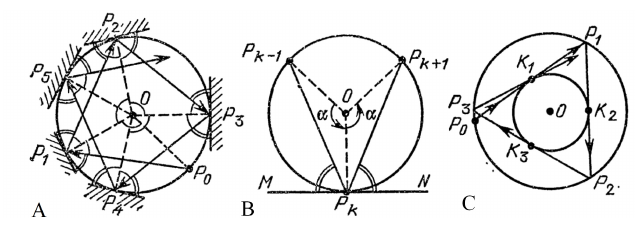
\includegraphics[width=0.9\textwidth]{bilard_kolowy.png}
\end{center}
\end{figure}    

Kąt $\beta$ jest zachowywany podczas odbić na podstawie prawa odbicia:
kąt padania jest równy kątowi odbicia. Tory w kolejnych odbiciach:
$P_{k-1}P_kP_{k+1}$ można wygenerowować przez obrót dowolnego wybranego toru,
np. $P_0P_1P_2$, o kąt $\alpha = \pi - 2\beta$ wokół środka okręgu.
ślad obracanych torów pozostawi "dziurę" w środku okręgu, której 
promień jest równy $R\sin\beta$, gdzie $R$ jest promieniem okręgu.
To oznacza, że trajektoria nie przechodzi przez każdy punkt przestrzeni fazowej,
więc ruch nie jest ergodyczny.

\newpage   
\end{solution}
%%%%%%%%%%%%%%%%%%%%%%%%%%%%%%%%%%%%%%%%%%%%%%%%%%%%%%%%%%%%%%%%%%%%%%%%%%%%
\zadanie[]

Proszę udowodnić twierdzenie Jacobiego: jeśli kąt $\alpha$  
jest niewspółmierny z $\pi$, kolejne punkty przecięcia trajektorii 
bilarda z okręgiem: $P_0, P_1, \ldots$
wypełniają ten okrąg w sposób gęsty, czyli w każdym odcinku łukowym 
o skończonej długości będzie przynajmniej jeden taki punkt.

\begin{solution}

Oznaczy położenie punktu $P_n$  przez kąt $\varphi_n$, 
liczony od pewnego ustalonego punktu odniesienia. W poprzednim zadaniu 
zauważyliśmy, że kolejne punkty odbicia powstają przez
obracanie punktu $P_0$ wokół środka okręgu o stały kąt $\alpha$. Zatem:
\begin{align*}
  \varphi_n = \varphi_0 + n\alpha 
\end{align*}
Musimy więc pokazać, że zbiór punktów
\begin{align*}
  \{\varphi_0 + n\alpha \pmod{2\pi} : n=0,1,2,\ldots\}
\end{align*}
jest gęsty na okręgu, gdy $\alpha/\pi$ jest liczbą niewymierną.
Położeniu punktu $P_0$ możemy przyjąć jako punkt odniesienia, 
więc bez straty ogólności możemy założyć, że $\varphi_0 = 0$.

Jeśli $\alpha$ jest współmierne z $\pi$, czyli $\alpha/\pi$ jest liczbą 
wymierną: $m/n$ to trajektoria będzie okresowa, z okresem $n$,
a punkty $P_0, P_1, \ldots P_{n-1}$  
będą znajdować się tylko w skończonej liczbie punktów na okręgu, więc nie 
będą gęste.



Weźmy dowolne $N \in \mathbb{N}$ i rozważmy $N+1$ punktów:
\begin{align*}
  0,\ \alpha,\ 2\alpha,\ \ldots,\ N\alpha \pmod{2\pi}.
\end{align*}
Podzielmy okrąg na $N$ łuków o równej długości $2\pi/N$. Na mocy zasady
szufladkowej Dirichleta dwa z powyższych $N+1$ punktów muszą wpaść do tego
samego łuku. Ich różnica ma więc postać
\begin{align*}
  \delta = m\alpha \pmod{2\pi}, \qquad 1 \le m \le N,
\end{align*}
oraz spełnia nierówność
\begin{align*}
  0 < \delta < \frac{2\pi}{N}.
\end{align*}
Lewa nierówność jest ścisła, bo z założenia $\alpha/\pi$ jest niewymierne,
więc nie istnieje takie całkowite $m \ne 0$, dla którego $m\alpha$ byłoby
wielokrotnością $2\pi$.

Rozważmy teraz punkty
\begin{align*}
  0,\ \delta,\ 2\delta,\ 3\delta,\ \ldots \pmod{2\pi}.
\end{align*}
Ponieważ krok $\delta$ jest mniejszy niż $2\pi/N$, to kolejne wielokrotności
$\delta$ rozmieszczają się na okręgu z odstępem nie większym niż $2\pi/N$.
Innymi słowy: w każdym łuku o długości większej niż $2\pi/N$ znajduje się
co najmniej jeden punkt postaci $l\delta \pmod{2\pi}$.

Ale każdy taki punkt ma postać
\begin{align*}
  l\delta = lm\alpha \pmod{2\pi},
\end{align*}
a więc jest jednym z punktów trajektorii $P_0,P_1,\ldots$.
Otrzymaliśmy zatem, że dla dowolnego $N$ w każdym łuku o długości większej niż
$2\pi/N$ leży pewien punkt trajektorii.

Teraz bierzemy dowolny niepusty łuk okręgu. Ma on pewną dodatnią długość $L$.
Wybieramy $N$ tak duże, aby $2\pi/N < L$. Wtedy w tym łuku musi znajdować się
co najmniej jeden punkt trajektorii. Ponieważ taki wybór można wykonać dla
każdego łuku o dodatniej długości, zbiór punktów $P_0,P_1,\ldots$ jest gęsty
na okręgu.

\newpage   
\end{solution}
%%%%%%%%%%%%%%%%%%%%%%%%%%%%%%%%%%%%%%%%%%%%%%%%%%%%%%%%%%%%%%%%%%%%%%%%%%%%
\zadanie[]

Proszę pokazać, że trajektoria bilardu jest gęsta w całym obszarze między brzegiem
bilardu ($\Gamma$) a okręgiem wewnętrznym $\gamma$.

\begin{solution}
    

\newpage   
\end{solution}
%%%%%%%%%%%%%%%%%%%%%%%%%%%%%%%%%%%%%%%%%%%%%%%%%%%%%%%%%%%%%%%%%%%%%%%%%%%%
%%%%%%%%%%%%%%%%%%%%%%%%%%%%%%%%%%%%%%%%%%%%%%%%%%%%%%%%%%%%%%%%%%%%%%%%%%%%
\zadanie[]

Proszę pokazać, że trajektoria bilardu jest ergodyczna na okręgu $\Gamma$.


\begin{solution}
    

\newpage   
\end{solution}
%%%%%%%%%%%%%%%%%%%%%%%%%%%%%%%%%%%%%%%%%%%%%%%%%%%%%%%%%%%%%%%%%%%%%%%%%%%%%%%
\zadanie[]

Rozpatrzmy pierwsze cyfry kolejnych potęg dwójki: 1, 2, 4, 8, 1, 3, 6, \ldots Czy w tym ciągu znajdzie się liczba 7?
Jeśli tak, to czy 7 czy 8 będzie występować częściej? A ogólniej, z jaką częstością będzie pojawiać się na początku
potęgi dwójki dany ciąg cyfr $a_1a_2\ldots a_r$?


\begin{solution}
    

\newpage   
\end{solution}
%%%%%%%%%%%%%%%%%%%%%%%%%%%%%%%%%%%%%%%%%%%%%%%%%%%%%%%%%%%%%%%%%%%%%%%%%%%%%%%%
\end{document}